\documentclass[a4paper, preprint, authoryear]{elsarticle} 

\usepackage{xr}
\externaldocument{../../paper/uniform}

\usepackage{pdfpages}
\usepackage[T2A]{fontenc}
\usepackage[utf8]{inputenc}
\usepackage[english]{babel}
\usepackage{amssymb,amsfonts,amsmath,mathtext,enumerate,float} 
\usepackage{mathtools}
\usepackage{amsthm}
\usepackage{graphicx, daytime} 
\usepackage{enumitem}
\usepackage[margin=1.6cm]{geometry}
\usepackage{environ}
\usepackage{listings}
\usepackage{lineno}
\usepackage{etoolbox}
\usepackage{multicol}
\usepackage{setspace}
\usepackage{array,caption}

\newtheorem{thm}{Theorem}
\newtheorem{lemma}{Lemma}
\newtheorem{corollary}{Corollary}
\newtheorem{property}{Property}

\renewcommand{\labelenumii}{\arabic{enumi}.\arabic{enumii}.}

\DeclarePairedDelimiter{\ceil}{\lceil}{\rceil}

\begin{document}
% Computational Approach
\section*{Appendix B. Computational Approach}

Since we do not have explicit formula for $B$, it is natural to find some computational approach. 
Then it is useful to propose an algorithm searching for the optimal $B$ 
with given $m, k, s$.
For example, we can try the following (approximation) algorithm to find worst-case performance $\hat{B} \geq B^{opt}$:

\subsection*{Algorithm with a grid search for $\varphi$}

\begin{enumerate}[itemsep = -1mm, leftmargin = *]

    \item Binary Search over $B$. Really, monotonous properties hold. As an upper bound we can take the Cho-Sahni result for the general case.

    \item Assume from now that $B$ is fixed. Check each $\varphi$ over a grid on the interval $[0, 1]$.

    \item Assume from now that $\varphi$ is fixed. Do binary search over $R$ for the third inequality from \eqref{scheme}.

    \item Here we assume that $R$ is fixed. Perform conditions check. Note that $z$ is obtained explicitly from $s$.

\end{enumerate}

Another option is to consider all possible $R$, then we do not need to do the 
grid search for $\varphi$. 

\subsection*{Optimization algorithm with iterating through the number of groups $R$}

\begin{enumerate}[itemsep = -1mm, leftmargin = *]
    \item Binary search over $B$ as in previous algorithm.

    \item Assume from now that $B$ is fixed. Do the following step for each $R$.

    \item The first inequality in \eqref{scheme} gives linear constraint 
        for $\varphi$. The third inequality in \eqref{scheme} is solved 
        by binary search over $\varphi$.

\end{enumerate}


From Property \ref{property-increase-m} it follows that  for fixed $s, k$ and running $m$ from 1 to infinity we may use the optimal result for
$m - 1$ as an upper bound for $B$, if the properties \ref{property-increase-m} hold.


\subsection*{Computation Results}


Here we present a plot of scheme quality for some parameters, and compare our results to the Cho-Sahni results.

        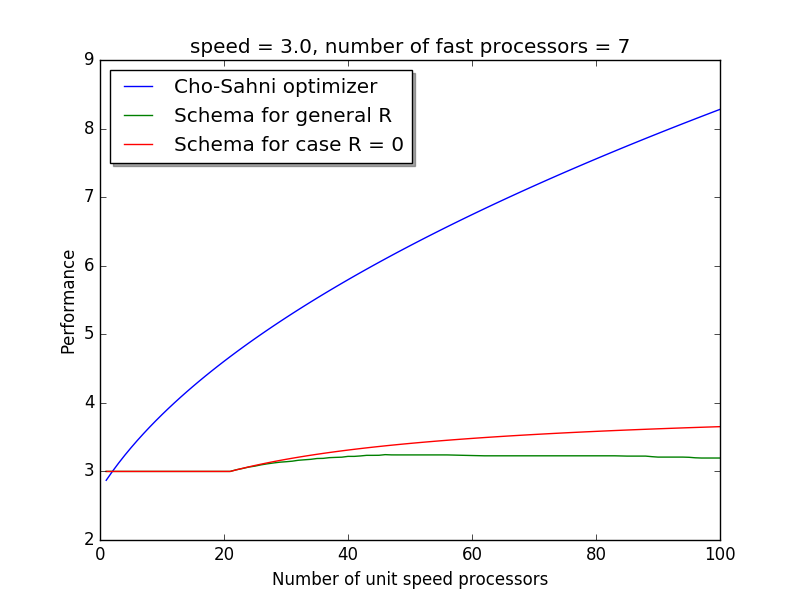
\includegraphics[scale = 0.35]{{./include/speed=3.0-fast=7}.png}
        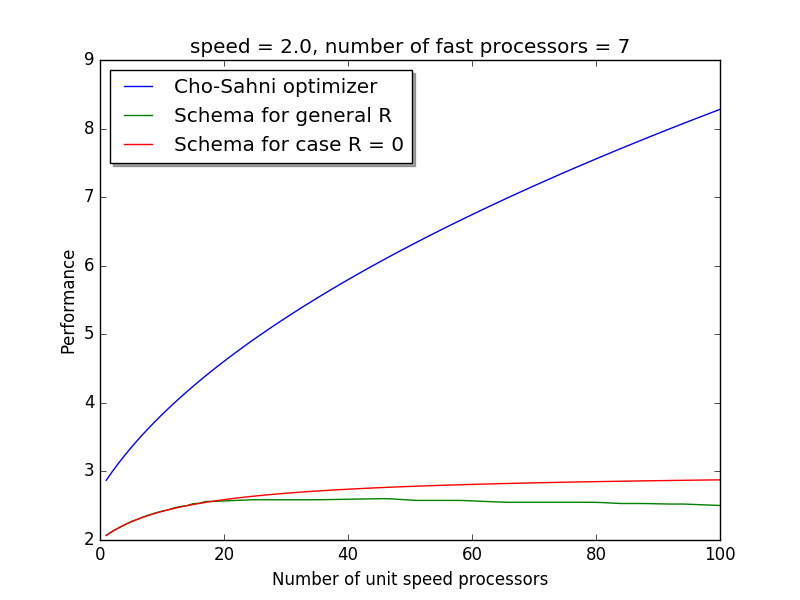
\includegraphics[scale = 0.35]{{./include/speed=2.0-fast=7}.png}


        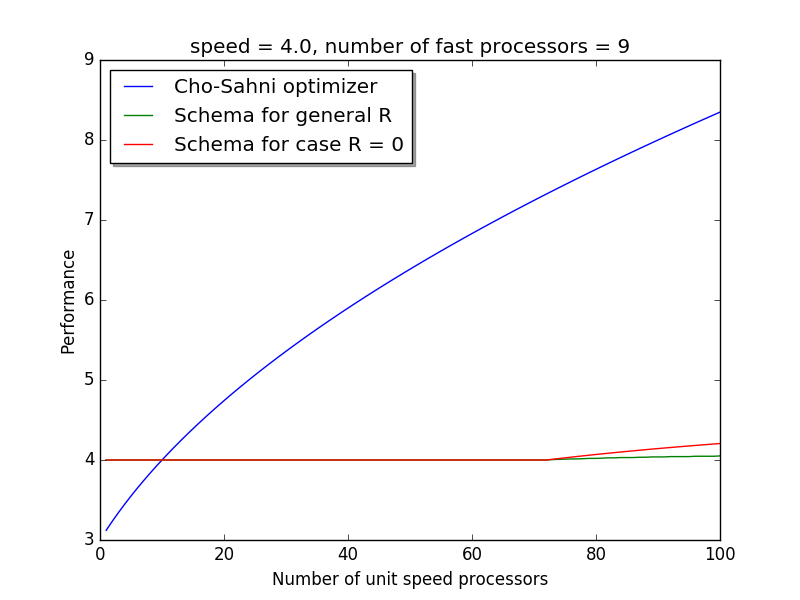
\includegraphics[scale = 0.35]{{./include/speed=4.0-fast=9}.png}
        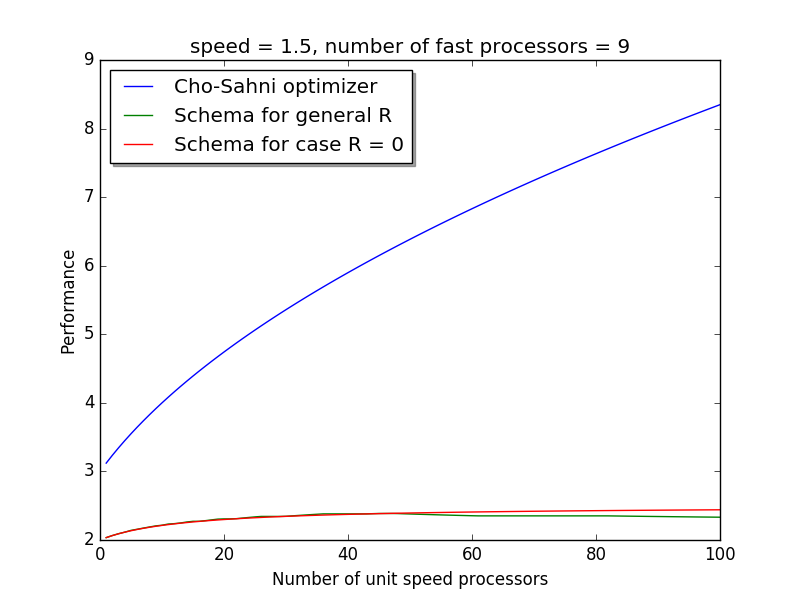
\includegraphics[scale = 0.35]{{./include/speed=1.5-fast=9}.png}

Levels plot for the difference in worst-case performance between our scheme and Cho-Sahni result.

        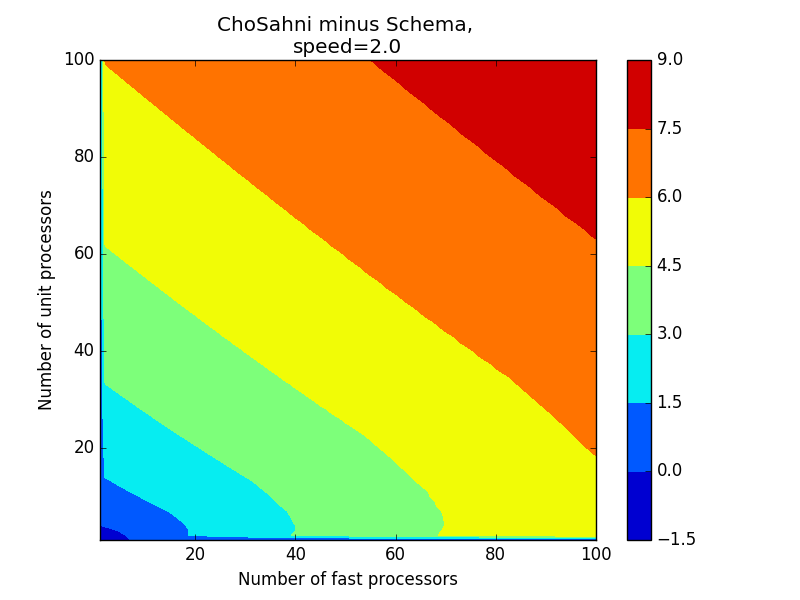
\includegraphics[scale = 0.35]{{./include/contour-speed=2.0}.png}
        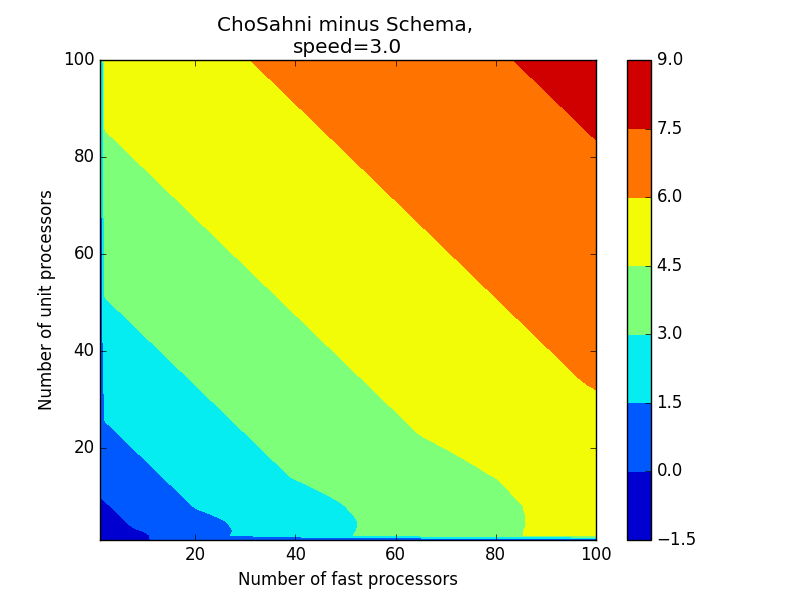
\includegraphics[scale = 0.35]{{./include/contour-speed=3.0}.png}

The table below illustrates performance of the scheme presented in the paper depending on the number of fast and normal machines when $s = 2$.

\begin{table*}[ht]
\tabcolsep=0.11cm
\tiny
\caption{Performance of Scheme} 
\label{performance-table}
\begin{tabular}{|c|c|c|c|c|c|c|c|c|c|c|c|c|}
\hline
head &  fast = 1 & fast = 2 & fast = 3 & fast = 4 & fast = 5 & fast = 6 & fast = 7 & fast = 8 & fast = 9 & fast = 10 & fast = 11 & fast = 12 \\ \hline
unit = 1 &
2.3364 & 2.2005 & 2.1452 & 2.1118 & 2.0916 & 2.0781 & 2.067 & 2.0599 & 2.0533 & 2.048 & 2.0436 & 2.0408 \\
\hline
unit = 2 &
2.5 & 2.3364 & 2.2508 & 2.2005 & 2.1696 & 2.1452 & 2.1277 & 2.1118 & 2.1018 & 2.0916 & 2.0833 & 2.0781 \\
\hline
unit = 3 &
2.5735 & 2.439 & 2.3364 & 2.2727 & 2.233 & 2.2005 & 2.177 & 2.1592 & 2.1452 & 2.1308 & 2.1219 & 2.1118 \\
\hline
unit = 4 &
2.5873 & 2.5 & 2.4096 & 2.3364 & 2.2901 & 2.2508 & 2.2222 & 2.2005 & 2.1834 & 2.1696 & 2.1544 & 2.1452 \\
\hline
unit = 5 &
2.5873 & 2.5625 & 2.4638 & 2.3864 & 2.3364 & 2.2989 & 2.268 & 2.2424 & 2.2222 & 2.2005 & 2.1875 & 2.1739 \\
\hline
unit = 6 &
2.5974 & 2.5735 & 2.5 & 2.439 & 2.381 & 2.3364 & 2.3004 & 2.2727 & 2.2508 & 2.233 & 2.2183 & 2.2005 \\
\hline
unit = 7 &
2.5882 & 2.5862 & 2.5435 & 2.4691 & 2.4129 & 2.3755 & 2.3364 & 2.3063 & 2.2824 & 2.2629 & 2.2467 & 2.2267 \\
\hline
unit = 8 &
2.5772 & 2.5873 & 2.5641 & 2.5 & 2.4476 & 2.4096 & 2.3684 & 2.3364 & 2.3109 & 2.2901 & 2.2727 & 2.2508 \\
\hline
unit = 9 &
2.5591 & 2.5873 & 2.5735 & 2.5316 & 2.4765 & 2.439 & 2.3964 & 2.3631 & 2.3364 & 2.3146 & 2.2964 & 2.2727 \\
\hline
unit = 10 &
2.5502 & 2.5873 & 2.5822 & 2.5625 & 2.5 & 2.4638 & 2.4204 & 2.3864 & 2.359 & 2.3364 & 2.3176 & 2.2989 \\
\hline
unit = 11 &
2.5502 & 2.5921 & 2.5873 & 2.5665 & 2.5316 & 2.484 & 2.4406 & 2.4096 & 2.381 & 2.3557 & 2.3364 & 2.3201 \\
\hline
unit = 12 &
2.5323 & 2.5974 & 2.5873 & 2.5735 & 2.5559 & 2.5 & 2.4691 & 2.439 & 2.4096 & 2.381 & 2.3529 & 2.3364 \\
\hline
unit = 13 &
2.526 & 2.6022 & 2.5873 & 2.5801 & 2.5625 & 2.5316 & 2.4894 & 2.4537 & 2.4245 & 2.4004 & 2.38 & 2.3529 \\
\hline
unit = 14 &
2.5105 & 2.5882 & 2.5873 & 2.5862 & 2.568 & 2.5435 & 2.5 & 2.4691 & 2.439 & 2.4129 & 2.3927 & 2.3755 \\
\hline
unit = 15 &
2.5036 & 2.5772 & 2.5873 & 2.5873 & 2.5735 & 2.5625 & 2.5294 & 2.4934 & 2.4638 & 2.439 & 2.4096 & 2.3864 \\
\hline
unit = 16 &
2.5036 & 2.5772 & 2.5902 & 2.5873 & 2.5788 & 2.5641 & 2.5346 & 2.5 & 2.4715 & 2.4476 & 2.4272 & 2.4096 \\
\hline
unit = 17 &
2.4882 & 2.572 & 2.5939 & 2.5873 & 2.5838 & 2.5689 & 2.5612 & 2.5258 & 2.4965 & 2.4691 & 2.439 & 2.4173 \\
\hline
unit = 18 &
2.4764 & 2.5591 & 2.5974 & 2.5873 & 2.5873 & 2.5735 & 2.5625 & 2.5316 & 2.5 & 2.4765 & 2.4564 & 2.439 \\
\hline
unit = 19 &
2.4764 & 2.5502 & 2.6007 & 2.5873 & 2.5873 & 2.5779 & 2.5655 & 2.5513 & 2.5229 & 2.4989 & 2.4691 & 2.4435 \\
\hline
unit = 20 &
2.4764 & 2.5502 & 2.6016 & 2.5873 & 2.5873 & 2.5822 & 2.5696 & 2.5625 & 2.5316 & 2.5 & 2.4806 & 2.4638 \\
\hline
unit = 21 &
2.4606 & 2.5502 & 2.5882 & 2.5892 & 2.5873 & 2.5862 & 2.5735 & 2.5629 & 2.5435 & 2.5207 & 2.5 & 2.4691 \\
\hline
unit = 22 &
2.4477 & 2.5502 & 2.5772 & 2.5921 & 2.5873 & 2.5873 & 2.5773 & 2.5665 & 2.5625 & 2.5316 & 2.5 & 2.484 \\
\hline
unit = 23 &
2.4477 & 2.5472 & 2.5772 & 2.5948 & 2.5873 & 2.5873 & 2.581 & 2.5701 & 2.5625 & 2.5373 & 2.5188 & 2.5 \\
\hline
unit = 24 &
2.4466 & 2.5323 & 2.5772 & 2.5974 & 2.5873 & 2.5873 & 2.5845 & 2.5735 & 2.5641 & 2.5559 & 2.5316 & 2.5 \\
\hline
unit = 25 &
2.4431 & 2.5323 & 2.5766 & 2.5999 & 2.5873 & 2.5873 & 2.5873 & 2.5769 & 2.5673 & 2.5625 & 2.5321 & 2.5172 \\
\hline
unit = 26 &
2.4311 & 2.526 & 2.5676 & 2.6022 & 2.5886 & 2.5873 & 2.5873 & 2.5801 & 2.5705 & 2.5625 & 2.5492 & 2.5316 \\
\hline
unit = 27 &
2.4202 & 2.5234 & 2.5591 & 2.5982 & 2.591 & 2.5873 & 2.5873 & 2.5832 & 2.5735 & 2.5651 & 2.5625 & 2.5316 \\
\hline
unit = 28 &
2.4165 & 2.5105 & 2.551 & 2.5882 & 2.5932 & 2.5873 & 2.5873 & 2.5862 & 2.5765 & 2.568 & 2.5625 & 2.5435 \\
\hline
unit = 29 &
2.4165 & 2.5036 & 2.5502 & 2.5788 & 2.5953 & 2.5873 & 2.5873 & 2.5873 & 2.5794 & 2.5708 & 2.5632 & 2.559 \\
\hline
unit = 30 &
2.4165 & 2.5036 & 2.5502 & 2.5772 & 2.5974 & 2.5873 & 2.5873 & 2.5873 & 2.5822 & 2.5735 & 2.5659 & 2.5625 \\
\hline
unit = 31 &
2.4138 & 2.5036 & 2.5502 & 2.5772 & 2.5994 & 2.5882 & 2.5873 & 2.5873 & 2.5849 & 2.5762 & 2.5685 & 2.5625 \\
\hline
unit = 32 &
2.401 & 2.5036 & 2.5502 & 2.5772 & 2.6013 & 2.5902 & 2.5873 & 2.5873 & 2.5873 & 2.5788 & 2.571 & 2.5641 \\
\hline
unit = 33 &
2.3964 & 2.497 & 2.5502 & 2.5772 & 2.6031 & 2.5921 & 2.5873 & 2.5873 & 2.5873 & 2.5813 & 2.5735 & 2.5665 \\
\hline
unit = 34 &
2.3881 & 2.4882 & 2.5499 & 2.572 & 2.5962 & 2.5939 & 2.5873 & 2.5873 & 2.5873 & 2.5838 & 2.576 & 2.5689 \\
\hline
unit = 35 &
2.3881 & 2.4798 & 2.5433 & 2.5654 & 2.5882 & 2.5957 & 2.5873 & 2.5873 & 2.5873 & 2.5862 & 2.5783 & 2.5713 \\
\hline
unit = 36 &
2.3881 & 2.4764 & 2.5323 & 2.5591 & 2.5806 & 2.5974 & 2.5879 & 2.5873 & 2.5873 & 2.5873 & 2.5806 & 2.5735 \\
\hline
unit = 37 &
2.3851 & 2.4764 & 2.5323 & 2.553 & 2.5772 & 2.5991 & 2.5896 & 2.5873 & 2.5873 & 2.5873 & 2.5829 & 2.5758 \\
\hline
unit = 38 &
2.3756 & 2.4764 & 2.5304 & 2.5502 & 2.5772 & 2.6007 & 2.5913 & 2.5873 & 2.5873 & 2.5873 & 2.5851 & 2.5779 \\
\hline
unit = 39 &
2.3714 & 2.4764 & 2.526 & 2.5502 & 2.5772 & 2.6022 & 2.5929 & 2.5873 & 2.5873 & 2.5873 & 2.5873 & 2.5801 \\
\hline
unit = 40 &
2.3714 & 2.4764 & 2.5243 & 2.5502 & 2.5772 & 2.6016 & 2.5944 & 2.5873 & 2.5873 & 2.5873 & 2.5873 & 2.5822 \\
\hline
unit = 41 &
2.3684 & 2.4698 & 2.519 & 2.5502 & 2.5772 & 2.5948 & 2.5959 & 2.5877 & 2.5873 & 2.5873 & 2.5873 & 2.5842 \\
\hline
unit = 42 &
2.3654 & 2.4606 & 2.5105 & 2.5502 & 2.5748 & 2.5882 & 2.5974 & 2.5892 & 2.5873 & 2.5873 & 2.5873 & 2.5862 \\
\hline
unit = 43 &
2.3654 & 2.4519 & 2.5036 & 2.5502 & 2.5693 & 2.5819 & 2.5988 & 2.5907 & 2.5873 & 2.5873 & 2.5873 & 2.5873 \\
\hline
unit = 44 &
2.3614 & 2.4477 & 2.5036 & 2.5502 & 2.5641 & 2.5772 & 2.6002 & 2.5921 & 2.5873 & 2.5873 & 2.5873 & 2.5873 \\
\hline
unit = 45 &
2.3614 & 2.4477 & 2.5036 & 2.5502 & 2.5591 & 2.5772 & 2.6016 & 2.5935 & 2.5873 & 2.5873 & 2.5873 & 2.5873 \\
\hline
unit = 46 &
2.3585 & 2.4477 & 2.5036 & 2.5472 & 2.5542 & 2.5772 & 2.6029 & 2.5948 & 2.5876 & 2.5873 & 2.5873 & 2.5873 \\
\hline
unit = 47 &
2.3524 & 2.4466 & 2.5036 & 2.5403 & 2.5502 & 2.5772 & 2.5997 & 2.5961 & 2.5889 & 2.5873 & 2.5873 & 2.5873 \\
\hline
unit = 48 &
2.3466 & 2.4466 & 2.5036 & 2.5323 & 2.5502 & 2.5772 & 2.5939 & 2.5974 & 2.5902 & 2.5873 & 2.5873 & 2.5873 \\
\hline
unit = 49 &
2.3435 & 2.4466 & 2.5 & 2.5323 & 2.5502 & 2.5772 & 2.5882 & 2.5987 & 2.5915 & 2.5873 & 2.5873 & 2.5873 \\
\hline
unit = 50 &
2.3407 & 2.4431 & 2.494 & 2.5323 & 2.5502 & 2.5766 & 2.5828 & 2.5999 & 2.5927 & 2.5873 & 2.5873 & 2.5873 \\
\hline
\end{tabular}
\normalsize
\end{table*}



\end{document}
